\documentclass{imc-inf}

\title{What is the Market Demand of AI and Big Data in Educational Market?}
\subtitle{Impact of AI and big data on educational institutes}
\thesistype{Bachelor Expos\'e}
\author{Ariunzaya Odontugs}
\supervisor{Rub\'en Ruiz Torrubiano}
\copyrightyear{2024}
\submissiondate{27.06.2024}
\keywords {Big Data, Artificial Intelligence, Educational Market, Machine Learning}



% \usepackage{xyz}
% ... add your own packages here!
\usepackage{listings}
\usepackage{subcaption}
                              

\begin{document}
\frontmatter\maketitle{}


\begin{declarations}\end{declarations}



\begin{abstract}
	The integration of AI and big data analytics into the world of education can be paradigm altering compared to the traditional methods of teaching and learning. The focus of this document will be on how this integration impacts institutional practices. Another point of focus is what the application of AI and big data are, what has already been done. Examine the implementations and consider the challenges and opportunities that arise. Furthermore, what is being done to mitigate it. 
	Overall it will go into detail about what current researches exist and what my experiment will do to find the impacts of the applications are on the educational market today. 
	
	
\end{abstract}


\addtoToC{Table of Contents}%
\tableofcontents%
\clearpage


\addtoToC{List of Figures}%
\listoffigures
\clearpage


%   MAIN MATTER  %%%%%%%%%%%%%%%%%%%%%%%%%%%%%%%%%%%%%%%%%%%%%%%%%%%%%%%%%%%%%%
\mainmatter%

\chapter{Introduction}\label{chap:introduction}

In this chapter I will introduce what Artificial Intelligence (AI) and big data mean in context of educational market. How they are being used to enhance learning and administrative processes. What the current trends are in the adoption of AI and Big Data in education. I will also introduce what my research method and approaches are. 

\section{Introduction and Motivation }
First of all, let’s start with what is big data. There has been debates on what the definition of big data is. Some have defined it as a large volume of data and others have a more detailed definition. For example, according to \cite{1} states that big data can be characterized with the “10 Bigs”. These characteristics are namely volume, big velocity, big variety, big veracity, big intelligence, big analytics, big infrastructure, big service, big value, and big market. If a dataset exhibits several of these characteristics that dataset can be considered as big data. Explaining and going into details of each of these characteristics are not in the scope therefore, from this point on when big data is referred to if means a dataset that qualifies at least a few of these characteristics. 


Data driven decision making is becoming more and more common as the data science field evolves throughout the years. Even though big data is not the solution to all problems in the educational field it can be used to create solutions and integrated into administrations and can be used as an aid in education among students of all ages. 


However, in regard to artificial intelligence which are algorithms that are inspired by how the human brain works I will research how these algorithms can be used in the educational market and how they can be used to solve problems in that focus. 

AI and big data can be used to automate some tasks such as grading which can be error prone and time consuming furthermore prone to human bias. In addition, some of the problems that AI and big data attempts to solve are personalized learning, in administrative tasks such as tracking student performance, scheduling, allocating resources, and grading and assessment. This can be useful in providing accuracy, efficiency and useful analytics that can aid in decision making. 

Artificial intelligence can also aid in automating students daily tasks such as note taking, studying, making flash cards and such tasks. These tasks are definitely time consuming and can be automated. By automating these tasks students can focus on the content more easily. Another advantage is that students have the ability to adapt these to their way of learning which is more effective for studying and tailor it to their needs. 

In recent studies there has been many uses of AI in helping children with mental and physical disorders to learn. There is research being done on whether the use of machine learning algorithms can aid in helping children with neurodevelopmental disorders. The research also goes into the limitations and future challenges that they might face. So, AI and big data are being utilized in ways we have not imagined before. 

Overall the integration of artificial intelligence and decision making based on big data can help with efficiency and effectiveness. 

\section{Research Problem }
There have been many studies done with the focus of artificial intelligence and big data separately. However, there are not enough studies done on how these topics affect the educational market together. How technology is being adopted and perceived by educational institutes is a topic needing much attention. Therefore, there is need to research this area further and analyze the impact of AI and big data on educational institutes. 

One of the issues in gathering data for this purpose is data protection regulation. Most of the AI systems will need user data and in order to function. The machine learning algorithms will need to be trained on user data. It will also generate an output based on the input of the user. Which can create copyright issues. This can be mitigated by the fact that there cannot be any reproducing and distributing of the generated material. However, we all know how these are very loose concepts that are only now coming into EU laws. 

There are also possible ethical issues that we might meet on the way. For example, privacy and security. If AI systems are being used in the administrative perspective there are vast amounts of data that is collected from students and lecturers that include personal information, academic integrity, academic performance and so on. All of this data is sensitive and can be a point of weakness in a data centric system. Therefore, ensuring the safety and security of the data and by extension the people behind the data becomes crucial. 

Another ethical issue is consent. How to collect a large amount of sensitive data from educational institutes and ensure their safety and security? Do the students know that their data can be used for training AI models. 

There is also another major issue that hinders the development and integration of AI in educational systems. It is the fact that not everything is perfect. While a majority of the world has access to resources such as internet, electricity, computers and in general technology, not everyone will be able to access these resources. Hence, if the educational institute decides to use such methods in their teachings, they must make sure that every person involved has access to such resources. Which of course is quite a challenging task. This is also the reason why some countries prefer sticking to simple methods of teaching and administrating educational tasks. Of course, this cannot be mitigated that easily. 


\section{Research Question }
My question involves researching the question: “What the market demand is for AI and big data are in the educational market?” There are many factors that are driving the adoption of AI and big data in education. First of all, computational power. Technological advancements are ever increasing every day. Which allows us to process and analyze vast amounts of data efficiently. Cloud computing solutions are now quite advanced that the processing and storing of such data are affordable. The processing power of machine learning algorithms has also increased significantly. 
Since the outbreak of Covid-19 we also know that “working from home” or for students “ learning from home” has become a concept that people are open to. We were in our DIY or “do it yourself” era. This opened a lot of possibilities in the sense that we do not always require a classroom to learn, and we do not always require an office to work. This could be one of the driving factors of remote style of learning and working. 

Another driving factor is the introduction of large language models such as Chat GPT, Llama and so on. When these systems were introduced a lot of other systems that used AI were introduced. Such as image generation, smart home systems and so on. Almost every market needed a new point of view regarding the use of AI and furthermore integration of them into their own systems. Especially in the educational market AI can be used for the greater good. 

This brings us to a debatable topic of: What do the educational institutions perceive the value and impact of AI and big data? There are a lot of controversial thoughts about this. Definitely understandable. One school of thought is that the use of AI such as Chat GPT is not advantageous for students. Of course, if AI is used not as a tool but as a shortcut it definitely will not benefit the user. However, not all uses can be identified as a shortcut and not all uses can be identified as not a shortcut. Therefore, an introduction of a system that enables students to take notes, or create quizzes, or create a study plan with the use of AI is needed, nevertheless. The use of Chat GPT is tricky for exam situations. However, if students are well prepared there should not be a need for using such methods. In order to prepare for such exams AI models could be quite useful. We can definitely see that AI is a part of everything nowadays so actually embedding these features into student lives instead of fighting it could provide useful. 

In order to study what the impacts would be I would like to determine from a dataset containing student information and the academic performances of those students before and after the use of AI. This will help to create an understanding of what the actual impacts are on the students. Which will help me to reflect on the impacts of it on education as a whole. 



\section{Research Method }
For my research method I would like to go into detail to try and find what the impact of AI in education actually looks like. There are collected data sets I can use to see the perception of AI from a student’s perspective and their performance. Which I can utilize to find out the general feeling towards AI and big data implemented in education. This is just to find out what trends are available in this data set. 

There are already data sets that contain student performance data, student behavioral data and data concerning age, gender and learning preferences, engagement data on how much time they spend on a specific activity. And using this data I would like to do data analysis to find the factors that explain the change or no change in performance of students, what kind of groups of students exist within the market and whether there are any obvious correlations between the features in the dataset. 





\section{Research Approach }
In this study, I will do analysis on data and use regression and clustering techniques to find the impact of AI on education especially on the perspective of students. 

\section{Structure}
This document outlines the details of the proposal for my Bachelor thesis. It contains the following structure. 
\begin{itemize}
	\item Chapter 1 focuses on the introduction where the motivation, Research Problem, Research Question, Research method, Research approach and the Structures are defined. 

	\item Chapter 2 contains the Background knowledge needed to understand the topic properly. Starting with Domain, Context, and Technology. 

	\item Chapter 3 goes into detail about the current state of the art (Related Works). It explains the Academic Research that was done and Commercial Products. 

	\item Chapter 4 is where the approach is explained in detail. It goes into Theoretical Background, explaining the data, data pre-processing,  experiment setup and evaluation. 

	 \item Chapter 5 is the summary of the expose. 

\end{itemize}


% Chapter 2
\chapter{Background}
Chapter 2 present some background information on the topic domain education, context and technology. 
\section{Education }
The main domain of my research is the application of AI and big data on the educational market. The broader domain is on teaching, learning and educational systems in general. What the impacts on teaching and learning will be when AI is integrated and making data driven decisions. The challenges and opportunities are discussed. 

\section{Artificial intelligence and big data }
Using advanced technology namely artificial intelligence and big data and analyzing how it can impact learning and teaching. For example, is the impact of using AI-driven personalized learning systems on the quality of learning and teaching. Can it improve engagement and keep students motivated? Would it fit unique needs of students?

Additionally, can AI and big data be used in administrative decision making processes to help lecturers and educational institutes to manage students and adapt the learning environment better tailored to them. For example, AI can be used to help develop curriculums based on historical data improve it to better suit students. That way you are always improving the curriculum which can be beneficial. 


\section{Technology }
The technologies used in the landscape of AI and Big data are wide and a lot of methodologies and frameworks. For the use of AI there are many machine learning algorithms that can be used. These machine learning algorithms are used for predictive analysis. For example, in our case there can be predictive models that are customized for each student. 

In addition, from the perspective of lecturers there can be automatic grading tools that will provide accurate and speedy results without human bias and errors. In regards to data using the latest big data processing frameworks such as Apache to handle volumes of data that a university or educational institute probably produces. Furthermore, there can be automatic analytics tools that can be used to get a better look into them. Which will definitely help the administrative processes. 




% Chapter 3
\chapter{Related Works}
In this I will go explain some of the existing academic research that has been done in the area of artificial intelligence and big data in regard to the educational market. Some details into what implementations exist already in the market. 

\section{Academic Research }
The adoption of online education has increased since the major impact of Covid-19 hit our lives. Since then, there has been investments made in order to improve the educational market. The main question is, how is that received among students?

There was a study in \cite{2} among 543 students of 5 different countries. The results differed country wise and gender wise. Some students without access to electricity, and the internet disliked the idea of involvement of tech in their education. Which is quite understandable. Some other students, while enjoying the more AI based adaptive learning systems however, faced some technical difficulties and were not offered sufficient help and support from instructors or the system. Which led them to try and find solutions on their own or with the help of their fellow students. In general, it seemed that even though some were satisfied with the solution of AI in education most were comfortable with the way they are studying now. 

This brings on a trade off between efficiency and ease. Even though there were major improvements and efficiencies in the use of AI in education is it worth it if it brings on more technical difficulties? Is that what is hindering the integration of such systems into the educational market? 
This is where big data can be useful. A collection and analysis of which areas students find challenging might help in determining improving points. For example, if it is a case of lacking in support with technical difficulties that can be mitigated by having a hybrid studying plan. Where people can enjoy the benefits of AI systems created with decision based on big data and have an in person classroom where support can be given. 

One of the papers I read introduced a very interesting viewpoint on the use of Chat GPT in the educational market. The paper \cite{3} goes into detail of using Chat GPT in education especially comparing media framing in Japan and Malaysia. Historically, it stated that Japan was not ready for the integration of technology  into education. The reason for this was for example outdated hardware, lack of technological support, and lack of effectiveness of tech on learning. The fact that Japan was not ready for tech integration was supported by the outbreak of Covid 19. Since then, the government has tried to include more technology into education by introducing initiatives to improve this through the years of 2019-2022. Malaysia on the other hand is having difficulties because of the lack and unreliability of internet connections, lack of device provision, absent teachers, and limited resources. They tried to mitigate the issue by also issuing government initiatives such as “Smart School”. They have been some success; however, they are still facing some challenges. Nevertheless, they are still committed out of most countries to keep trying since 3.9\% of their GDP is allocated for the department of education. 

One of the interesting things from this \cite{3} is the difference in perspectives of both countries. Japanese educators were optimistic about the integration of AI tools such as Chat GPT in education. Yet they worried that there might be a change in the motivation of students. Whereas Malaysian educators worried that the quality of education might be affected severely. The paper talks about how the viewpoint of AI tools varied from the type of stakeholder. Depending on whether you are a student, politician, or educator their perspectives drastically changed. Some are viewing AI tools such as Chat GPT as a threat to traditional learning methods. The paper also stresses the point that these views are very much shaped and colored by the outlook of media. The main source of people’s opinions has the tendency to be shaped by the public’s opinions and impact their final thoughts on the matter. For example, Malaysia has stated that Chat GPT in education might be revolutionary. On the other hand, Japan’s viewpoints mainly stem from overseas news and their standpoint is that they are not that impressed by what Chat GPT has to offer. Their main concerns revolve around the fact that the hyped-up AI tool will lead to a decrease and eventually absence of creative and critical thinking, while promoting laziness, cheating and lessen the importance of academic integrity. Regarding the overall tones of the media Malaysia was quite positive about the use of AI in particular Chat GPT and Japan had more negative tones about it. Keep in mind that those tones come from different stakeholders. For example, the positive tones of Malaysia stem from quotes from different media sources. Whereas Japan’s stem from the responses of the industry leaders. 
Overall, this paper states that there is a dire need for educators and policy makers to discuss the risks and implications of AI tools in education. Whether stakeholders agree or not there is a need for a major discussion to create methods that ensure the academic integrity of scholars. The situation seems like it is quite simple, however paints quite a complex picture. People also worry about the ethical implications and try to figure out ways how it’s best to mitigate those. Especially since the opinions about the use of AI in education are so divided, for example among just two countries Japan and Malaysia, it for sure will be a lot more divided when more countries get involved. This will definitely spark the need of an overall regulation for the usage of AI in education. 



\section{Commercial Products }
Currently one of the implementations of AI in education is LeewayHertz’s generative AI platform called ZBrain. This platform uses client data and large language models such as GPT-4, Vicuna, Llama 2, or GPT-Neox and develops tailored materials, personalized lesson plans, stories, worksheets, and quizzes. It promotes personalized learning and adaptive learning paths. This way using artificial intelligence solutions opens doors to optimize learning and help student’s efficiencies. 
This solution alleviates major problems that students face. For instance, planning, staying engaged and motivated. Since the AI solution targets student’s problems specifically, they will be more motivated to keep learning. 

Other existing implementations of AI in education actively being used by students is speech recognition algorithms to transcribe speech to text. This helps students to create notes of lectures for future independent studies. Instead of trying to take notes to keep up with the lecturer’s speech the student is able to focus on the lecture and let the transcriber do it’s job and create notes without any extra hassle. 

Another great example of AI implementation in the field of education from the perspective of students is apps such as “Penseum”. This app allows users to upload slides and notes onto it and the app will create a study schedule according to the provided data. It will create summaries of the lessons according to the slides along with multiple choice quizzes from the slides. It also creates flashcards automatically. This type of app really helps to save time for students and use learning styles best suited for them. For example, some learn best with flashcards and memorize while others benefit from a more Socratic approach with quizzes and questions. I personally have used this app and it saved me a lot of time and it was an easy and interesting way to learn. 

Upon research I read a paper on the applications of AI \cite{4} on education there was another implementation that interested me. The paper states that Computer-based training (CBT) and computer-aided instruction (CAI) were implemented over two decades ago. They utilized scripted decision-making processes that did not personalize instructions to individual learner needs or abilities. Therefore, they came up with the "Intelligent tutoring systems" or ITS. These systems achieve flexibility in material presentation and responsiveness to individual student needs. Because of their adaptive and flexible style they have been effective in improving student motivation and performance. 

Overall, it was interesting to see the different implementations and their different complexities among them. Furthermore, there has been a lot of successful implementations and integration of AI into education. 










% Chapter 4
\chapter{Approach}
Chapter 4 goes into detail and explains the methods I will use, details about the data, data pre-processing, what the experimentation stage looks like and finally the evaluation. 


\section{Theoretical Background }
In recent years, the integration of Artificial Intelligence (AI) and Big Data technologies into educational settings has sparked a lot of interest and definitely some debate. AI is characterized by its ability to simulate human intelligence through machine learning algorithms and neural networks, offers a lot of opportunities for assisting in learning, teaching and administrative work.

\subsection{Method 1: Descriptive Analysis}
In this method I would need to understand the details of my data. That can help me to get a better understanding of the features of my dataset. Descriptive analysis includes looking at the 5-point summaries of the data which are mean, median, mode, max, and mins of all of the features. Measure the variance and ranges of the data features. As an example, this would be useful for seeing the average grades of the students before and after AI integration. 

To better see the distribution of the dataset plotting and visualization is quite important. Using plots like boxplot, and plots to see the distribution of the categorical variables, using violin plots, and such are useful as well. 

\subsection{Method 2: Cluster Analysis}
Cluster analysis can be used to see if different stakeholders have different perspectives. Cluster analysis can help to see the underlying formations of groups between different stakeholders. Some methods of clustering are K-means, hierarchical clustering, and density-based clustering. I am planning on using density-based blustering because it is better at capturing complex shapes of groups. 

\subsection{Method 3: Regression Analysis}
Another method is regression analysis. These methods can be used to identify and understand the relationships between variables in the data sets and predict certain outcomes. For example, which features contribute the most in predicting student performance? Using regression or also multiple regression which allows the examination of multiple variables on the predictor variables we can identify the factors that are most significant and contribute to the predictor variables. 

\section{Data}
In the data collection stage, I would need to gather a comprehensive set of quantitative and qualitative data that can provide insights into different aspects of educational performance. In order to analyze the impact, I would need data from before and after the use of AI. We can also use data from educational institutes that track student progress which would provide valuable information. From these data sets we can then analyze the impact by looking at the performance metrics, plagiarism speculations, integrity of submitted assignments vs grade scores and so on. 

Some of the valuable information needed in the data set is performance metrics. Historical data on grades, assignment scores, completion percentages and dropout rates. Some of these metrics like completion percentages can be calculated so if the data set contained the number assignments per semester, that would also provide valuable information. Using these metrics, I can then analyze the potential changes that were prominent when AI was introduced. This can help to see what the impacts of AI are regarding performance. 

The plagiarism rate or a feature in the data set that contains information about the integrity of uploaded assignments and exams can also provide quite interesting information. Since one of the major concerns of the integration of AI in education is that the quality of works would decrease, it would be great to analyze that and prove whether that actually is the case. 

Another feature that the dataset should contain is the engagement score. Another main challenge that AI introduces in education is decreased motivation in students. In order to study and analyze this a feature like engagement would be useful. This could be for example an ordered variable that has choices such as 1-5 with 1 being not engaged at all and 5 being the most engaged. This could help identify whether motivation in courses is being affected by the introduction of AI. 

Additionally, having an extra data set just containing the perspectives of students and lecturers towards AI in education can provide valuable information. With it I can analyze potential groupings in stakeholders. Identify whether a certain group’s perspective is more prevalent than another group. This could help to illustrate how AI is being perceived among different stakeholders. 

Overall, there are a lot of data features needed for detailed analysis, however, these can be analyzed separately when needed. This would also help to clearly see certain trends as well. Data regarding students’ perception of AI already exists \cite{5}. Data regarding student performances I am still in pursuit of. 

\section{Pre-processing}
There are a few crucial steps for the pre-processing stage. Those stages are the following:
\begin{enumerate}
	\item Data cleaning: \\
	
	As with all data sets there probably will be noise, and empty values, outliers and such. In order to have a clean data set that produces the most reliable outcomes we need to handle these. Depending on how many rows are missing either remove or impute the missing values. If its just a few out of 10,000 rows of data then those rows can be removed. However, if there is a significant chunk of missing values then removing would be a waste of other good data. In tha case replacing them with values such as “Unknown” can actually provide good informational value. Sometimes missing information is valuable information. Another step in the data cleaning can include removing duplicates and handling outliers. 
	
	\item Data integration:\\
	I am most certain that I will need to use different sources of data. So data integration can be a tricky and important part of the data pre-processing stage. If data sets are combined I would need to take care that the data follows somewhat similar styles through the whole data set. This means making sure that data units are roughly the same across the whole data set. Which is important for regression analysis. 
	
	\item Data transformation:\\
	We need to normalize the data to scales that are similar to each other. Especially for clustering and regression standardization or normalization is an important step. I am also expecting there to be quite a lot of categorical variables. For these to be used in regression models will need to be encoded into numerical variables either by one-hot encoding or other techniques. 
	
	
\end{enumerate}

\section{Experiment setup}
For my implementation I will be using R programming to pre-process and do my coding. One of my data sources are Kaggle. It’s a data set on the perspective of students on using AI in education. My other data sets will have to be collected. I still need to find a proper data set on historical data on the performance of students. There are datasets on student performance open for use however I would like find a data set from a real university and get permission for use. 

Figure 1 depicts the steps of my research how I will reach evaluation step. 


\begin{figure}[h]
	\centering
	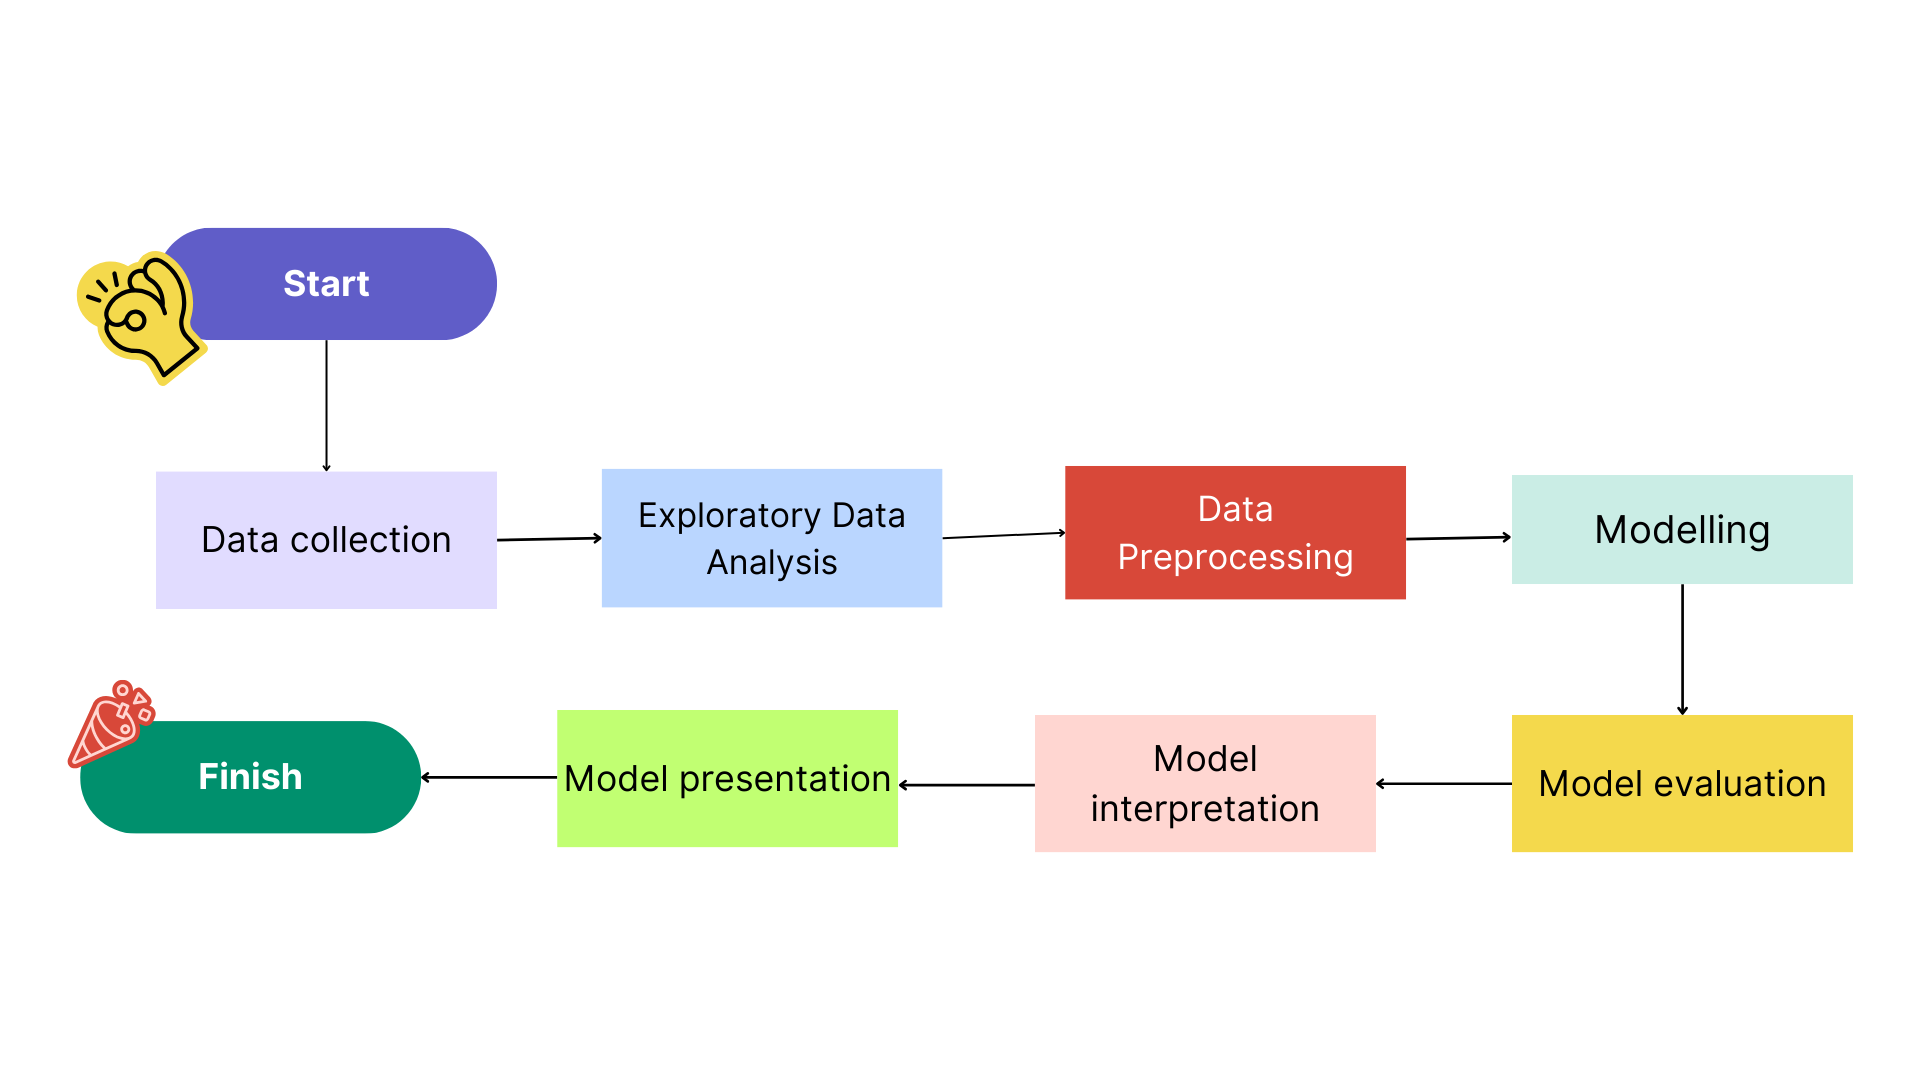
\includegraphics[width=1.0\textwidth]{Data-collection.png}
	\caption{Research plan diagram}
	\label{fig:example}
\end{figure}

\section{Evaluation}
For evaluating AI and Big data models in regards to the educational marketing especially in regards to clustering, metrics such as accuracy, precision, recall, and F1-scores can help assess predictive models. 

For regression tasks, mean absolute error (MAE) and mean squared error (MSE) quantify the average deviation of predicted outcomes from actual values. 

Additionally evaluation by visualization can be achieved by using ROC which stands for receiver operating characteristic curve (very exciting names :)) and AUC scores which stand for area under the curve. These we learned in our machine learning lecture. They can provide useful in finding an aggregate measure of performance across all possible classification thresholds. For example, ROC curve evaluates the trade-off between true positive rate and false positive rates. 

Using these metrics I will try and determine the impact of AI and big data in education. 

% Chapter 5 
\chapter{Summary}
In conclusion my experiment will analyze the impact of the usage of AI into education. We have seen that though there can be challenges such as ethical issues, educational institutes disapproving of the use of AI and limitation of resources there are also some benefits of using it. It can possibly be helpful in learning and improving performance of students. It can also be useful in the aspect of administrative ways. This impact will be researched through my experiment. 

Regardless of how much challenges there are, as there always are with evolving fields, it can provide to be an enhancement to education and open many possibilities. Therefore, looking at the impacts are crucial to be able to improve existing systems and create inclusive regulations. Especially if the integration is a popular implementation and is adopted popularly. Theses regulations can help with securing the safety of academic integrity while still being able to provide a paradigm shifting enhancement to education. 



\backmatter%
	\addtoToC{Bibliography}
	\bibliographystyle{IEEEtranS}
 \typeout{}
	\bibliography{references}
	

	‌
	


\end{document}
